%%%%%%%%%%%%%%%%%%%%%%%%%%%%%%%%%%%%%%%%%%%%%%%%%%%%%%%%%%%
% Full LaTeX Draft - V13 (Re-applied Figure Inclusion and Fixes)
%%%%%%%%%%%%%%%%%%%%%%%%%%%%%%%%%%%%%%%%%%%%%%%%%%%%%%%%%%%
\documentclass{article}

% Using the 'final' option from neurips_2019 for formatting
\usepackage[final]{neurips_2019} % Default natbib loading

\usepackage[utf8]{inputenc} % allow utf-8 input
\usepackage[T1]{fontenc}    % use 8-bit T1 fonts
\usepackage{hyperref}       % hyperlinks
\usepackage{url}            % simple URL typesetting
\usepackage{booktabs}       % professional-quality tables
\usepackage{amsfonts}       % blackboard math symbols
\usepackage{amssymb}        % For math symbols like \mathbb
\usepackage{nicefrac}       % compact symbols for 1/2, etc.
\usepackage{microtype}      % microtypography
\usepackage{graphicx}       % Required for including images
\usepackage{amsmath}        % For math formulas
\usepackage{placeins}       % To control float placement with \FloatBarrier
% \usepackage{natbib} % Let neurips_2019 handle this
\bibliographystyle{plainnat} % Define citation style

% Ensure hyperref setup is compatible
\hypersetup{
    colorlinks=true,        % Enable colored text links
    linkcolor=red,          % Internal links color (references, TOC) set to red
    filecolor=magenta,      % File links color
    urlcolor=cyan,          % URL links color
    citecolor=blue          % Citation links color kept as blue
}
\urlstyle{same}

% --- Your TITLE ---
\title{Comparative Analysis of Manifold Learning Methods for Face Pose Ordering}

% --- Your AUTHORS --- (Using \& for ampersands)
\author{%
  Ding Ding \\
  Department of Mathematics\\
  The Hong Kong University of Science and Technology\\
  \texttt{ddingab@ust.hk} \\
  \And
  Zihao Zhang \\
  Department of Mathematics\\
  The Hong Kong University of Science and Technology\\
  \texttt{zzhangjn@ust.hk} \\
  \And
  Bingsong Gao \\
  Department of Mathematics\\
  The Hong Kong University of Science and Technology\\
  \texttt{bgaoaj@ust.hk} \\
}

\begin{document}

\maketitle

% --- Your ABSTRACT ---
\begin{abstract}
  Recovering the underlying low-dimensional manifold structure from high-dimensional data, such as images, is a fundamental task in machine learning and data analysis. This project investigates the effectiveness of various dimensionality reduction techniques in recovering the 1D rotational pose manifold from a dataset of 33 grayscale face images of the same individual viewed from different angles. We applied nine methods: Principal Component Analysis (PCA), Multidimensional Scaling (MDS), Isomap, Locally Linear Embedding (LLE), Local Tangent Space Alignment (LTSA), Modified LLE (MLLE), Hessian LLE (HLLE), Spectral Embedding, and t-Distributed Stochastic Neighbor Embedding (t-SNE). Performance was evaluated based on the accuracy of pose ordering using Total Absolute Error (TAE) relative to a visually refined ground truth sequence, as well as standard metrics for local structure preservation, namely Trustworthiness (T) and Continuity (C). Key hyperparameters, specifically the number of neighbors ($k$) for neighbor-based methods and perplexity ($p$) for t-SNE, were systematically tuned. Our results indicate that Isomap (k=5) achieved the best ordering performance (TAE=6), closely followed by LLE (k=5, TAE=14), Spectral Embedding (k=5, TAE=14), HLLE (k=10, TAE=16), and LTSA (k=10, TAE=16). Most methods exhibited high Trustworthiness and Continuity, although some trade-offs were observed. The analysis highlights the importance of parameter selection and the influence of the ground truth definition on quantitative ordering metrics. t-SNE and MDS performed poorly in recovering the global pose order for this specific task and ground truth. The project code is available at \url{https://github.com/dingding-ust/manifold-learning-face-pose/tree/main}.
\end{abstract}

% --- Your INTRODUCTION ---
\section{Introduction}
\label{sec:intro}

Dimensionality reduction is a crucial preprocessing step when dealing with high-dimensional datasets prevalent in fields like computer vision, bioinformatics, and natural language processing. These datasets often exhibit intrinsic low-dimensional structures, or manifolds, hidden within the high-dimensional observation space. Manifold learning algorithms aim to uncover these underlying structures, providing compact representations that facilitate visualization, clustering, and classification tasks \citep{vanDerMaaten2009}. Applications range from visualizing complex biological data to estimating object pose from images \citep{Tenenbaum2000, Roweis2000}.

This project focuses on a classic manifold learning problem: recovering the underlying pose manifold from a collection of face images. We utilize a well-known dataset comprising 33 grayscale images of a single individual captured under varying horizontal viewpoints \citep{Tenenbaum2000}. The intrinsic structure is expected to be a one-dimensional manifold corresponding to the continuous head rotation. The primary goal is to evaluate and compare the ability of various linear and non-linear dimensionality reduction techniques to capture this 1D manifold and accurately order the face images according to pose.

We employ a suite of nine dimensionality reduction methods, including the linear baseline methods Principal Component Analysis (PCA) and classical Multidimensional Scaling (MDS), as well as prominent non-linear manifold learning algorithms: Isomap \citep{Tenenbaum2000}, Locally Linear Embedding (LLE) \citep{Roweis2000}, Local Tangent Space Alignment (LTSA) \citep{Zhang2004}, Modified LLE (MLLE) \citep{Zhang2007}, Hessian LLE (HLLE) \citep{Donoho2003}, Spectral Embedding \citep{Belkin2003}, and t-Distributed Stochastic Neighbor Embedding (t-SNE) \citep{vanDerMaaten2008}.

To quantitatively assess the performance, particularly for the ordering task, we established a ground truth sequence based on visual inspection and refinement. We evaluate the methods using the Total Absolute Error (TAE) metric, which measures the deviation of the algorithm-induced order (derived from the primary embedding dimension) from the ground truth. Additionally, we employ Trustworthiness (T) and Continuity (C) metrics \citep{Venna2001} to evaluate the preservation of local neighborhood structures in the 2D embeddings. Recognizing the sensitivity of manifold algorithms to hyperparameters, we perform systematic parameter tuning for the number of neighbors ($k$) in neighbor-based methods and perplexity ($p$) for t-SNE, analyzing their impact on the evaluation metrics through visualizations.

This report is structured as follows: Section \ref{sec:dataset} describes the dataset and ground truth establishment. Section \ref{sec:methods} reviews the dimensionality reduction methods employed in detail. Section \ref{sec:setup} details the experimental setup and evaluation metrics. Section \ref{sec:results} presents and discusses the results. Finally, Section \ref{sec:conclusion} concludes the report.

% --- Your DATASET Section ---
\section{Dataset and Ground Truth}
\label{sec:dataset}

The primary dataset used consists of 33 grayscale images ($N=33$) of a single individual's face, captured from varying horizontal viewpoints. Each image is $92 \times 112$ pixels (Height $\times$ Width). Flattened, each image $\mathbf{x}_i$ is a point in $\mathbb{R}^{D}$ where $D=10304$. The data lies on an approximate 1D manifold corresponding to head rotation \citep{Tenenbaum2000}. Figure \ref{fig:sample_faces} shows sample images.

\begin{figure}[htbp]
  \centering
  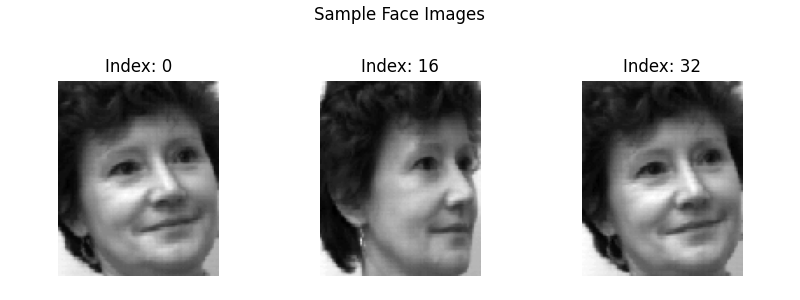
\includegraphics[width=0.8\linewidth]{../figs/sample_faces.png} % Using relative path
  \caption{Sample images (Indices 0, 16, 32) from the face pose dataset.}
  \label{fig:sample_faces}
\end{figure}

A ground truth sequence for pose ordering was established via visual inspection and refinement: [9, 20, 22, 14, 10, 4, 7, 0, 32, 13, 19, 12, 1, 30, 26, 11, 8, 5, 2, 29, 15, 16, 25, 21, 31, 17, 23, 6, 24, 27, 28, 3, 18] (0-based indices). The subjectivity of visual ordering is acknowledged.

%%%%%%%%%%%%%%%%%%%%%%%%%%%%%%%%%%%%%%%%%%%%%%%%%%%%%%%%%%%%%%%%%%%%%%
%   Section 3  —  Methods (Improved Formatting - V7)
%%%%%%%%%%%%%%%%%%%%%%%%%%%%%%%%%%%%%%%%%%%%%%%%%%%%%%%%%%%%%%%%%%%%%%
\section{Methods}\label{sec:methods}

We employed nine dimensionality reduction techniques mapping $\mathbf{X} = \{\mathbf{x}_i \in \mathbb{R}^D\}_{i=1}^N$ to $\mathbf{Y} = \{\mathbf{y}_i \in \mathbb{R}^d\}_{i=1}^N$ ($d=2$), using Scikit-learn \citep{scikit-learn}. Let $X$ be the $N \times D$ data matrix.

\subsection{Linear Methods}

\subsubsection{Principal Component Analysis (PCA)}
PCA identifies principal components maximizing data variance via linear projection \citep{Hotelling1933}. Assuming centered data $X_c$, it computes the covariance matrix $\mathbf{C} \propto X_c^T X_c$. The principal components are the eigenvectors $\mathbf{v}_j$ of $\mathbf{C}$ satisfying $\mathbf{C}\mathbf{v}_j = \lambda_j \mathbf{v}_j$. The embedding $\mathbf{Y}$ is obtained by projecting onto the top $d$ eigenvectors $\mathbf{V}_d = [\mathbf{v}_1, ..., \mathbf{v}_d]$:
\[ \mathbf{Y} = X_c \mathbf{V}_d \]

\subsubsection{Multidimensional Scaling (MDS)}
Classical MDS \citep{Young1941_MDS} reconstructs coordinates from pairwise dissimilarities $\delta_{ij}$. Using squared Euclidean distances $D_{ij} = \delta_{ij}^2 = ||\mathbf{x}_i - \mathbf{x}_j||^2$, the centered Gram matrix $\mathbf{B}$ is obtained via double centering:
\[ \mathbf{B} = -\frac{1}{2}\mathbf{H}\mathbf{D}^{(2)}\mathbf{H}, \quad \text{where } \mathbf{H} = \mathbf{I} - \frac{1}{N}\mathbf{1}\mathbf{1}^T \]
From the eigendecomposition $\mathbf{B} = \mathbf{U}\mathbf{\Lambda}\mathbf{U}^T$, the embedding coordinates are $\mathbf{Y} = \mathbf{U}_d \mathbf{\Lambda}_d^{1/2}$, using the top $d$ positive eigenvalues $\mathbf{\Lambda}_d$ and corresponding eigenvectors $\mathbf{U}_d$.

\subsection{Non-Linear Manifold Learning Methods}

\subsubsection{Isomap}
Isomap \citep{Tenenbaum2000} estimates geodesic distances using graph shortest paths. First, a $k$-nearest neighbor ($k$-NN) graph $G$ is constructed with edge weights $d(\mathbf{x}_i, \mathbf{x}_j)$. Second, all-pairs shortest path distances $\delta_{G}(i, j)$ are computed on $G$, forming the matrix $\mathbf{D}_G^{(2)} = [\delta_{G}(i, j)^2]$. Third, classical MDS is applied to $\mathbf{D}_G^{(2)}$ (using $\mathbf{B}_G = -\frac{1}{2}\mathbf{H}\mathbf{D}_G^{(2)}\mathbf{H}$) to obtain the embedding $\mathbf{Y}$. Depends on $k$.

\subsubsection{Locally Linear Embedding (LLE)}
LLE \citep{Roweis2000} preserves local linear reconstructions. First, for each $\mathbf{x}_i$, its $k$ nearest neighbors $\mathcal{N}_k(i)$ are identified. Second, weights $W_{ij}$ minimizing the local reconstruction error are found:
\[ \min_{W} \sum_{i=1}^N ||\mathbf{x}_i - \sum_{j \in \mathcal{N}_k(i)} W_{ij} \mathbf{x}_j||^2 \quad \text{s.t.} \sum_{j \in \mathcal{N}_k(i)} W_{ij} = 1 \]
This involves solving a constrained least-squares problem for each $i$. Third, the embedding $\mathbf{Y}$ is found by minimizing the cost $\Phi(Y) = \sum_i ||\mathbf{y}_i - \sum_{j} W_{ij} \mathbf{y}_j||^2 = \text{Tr}(\mathbf{Y}^T \mathbf{M} \mathbf{Y})$, where $\mathbf{M} = (\mathbf{I}-\mathbf{W})^T(\mathbf{I}-\mathbf{W})$. The solution uses the bottom $d$ non-zero eigenvectors of $\mathbf{M}$. Depends on $k$.

\subsubsection{Local Tangent Space Alignment (LTSA)}
LTSA \citep{Zhang2004} aligns local tangent spaces. For each neighborhood $\mathbf{X}_i$, it finds the tangent basis $\mathbf{V}_i$ via local PCA and computes local coordinates $\mathbf{\Theta}_i = \mathbf{V}_i^T (\mathbf{X}_i - \bar{\mathbf{x}}_i \mathbf{1}_k^T)$. It then seeks the global embedding $\mathbf{Y}$ by minimizing the alignment error:
\[ \sum_i || (\mathbf{Y}_i - \mathbf{y}_i\mathbf{1}_k^T) - \mathbf{L}_i \mathbf{\Theta}_i ||_F^2 \]
where $\mathbf{L}_i$ is a local affine transformation. This involves an eigenvalue problem on a global alignment matrix. Depends on $k$.

\subsubsection{Modified LLE (MLLE)}
MLLE \citep{Zhang2007} stabilizes LLE using multiple weight vectors $W_i$ per neighborhood, based on the local covariance null space. The embedding $\mathbf{Y}$ minimizes the sum of reconstruction errors using these weights:
\[ \min_{Y} \sum_{i} \text{Tr}( (\mathbf{Y}_i - \mathbf{y}_i \mathbf{1}_k^T)^T (\mathbf{Y}_i - \mathbf{y}_i \mathbf{1}_k^T) \mathbf{W}_i \mathbf{W}_i^T ) \]
Solved via eigendecomposition. Depends on $k$.

\subsubsection{Hessian LLE (HLLE)}
HLLE \citep{Donoho2003} uses local Hessian estimates $\mathcal{H}_i$. The embedding $\mathbf{Y}$ minimizes the integrated squared Hessian norm:
\[ \min_{Y} \sum_i || \mathcal{H}_i \mathbf{Y} ||^2 \approx \min_{Y} \text{Tr}(\mathbf{Y}^T \mathbf{K} \mathbf{Y}) \]
solved via eigenvectors of the kernel matrix $\mathbf{K}$ built from Hessian estimates. Requires $k > d(d+3)/2$. Depends on $k$.

\subsubsection{Spectral Embedding (Laplacian Eigenmaps)}
Based on graph spectral theory \citep{Belkin2003}. A $k$-NN graph with adjacency $\mathbf{W}$ is built. The graph Laplacian $\mathbf{L} = \mathbf{D} - \mathbf{W}$ is computed. The embedding $\mathbf{Y} = [\mathbf{v}_1, ..., \mathbf{v}_d]$ consists of the eigenvectors corresponding to the $d$ smallest non-zero eigenvalues of the generalized eigenproblem $L\mathbf{v} = \lambda D\mathbf{v}$. Depends on $k$.

\subsubsection{t-Distributed Stochastic Neighbor Embedding (t-SNE)}
Visualizes similarity \citep{vanDerMaaten2008}. It computes high-dimensional ($p_{ij}$) and low-dimensional ($q_{ij}$) joint probabilities representing pairwise similarities, using Gaussian and t-distributions respectively. $p_{ij}$ depends on the `perplexity` $p$.
\[ q_{ij} = \frac{(1 + ||\mathbf{y}_i - \mathbf{y}_j||^2)^{-1}}{Z} \]
It minimizes the KL divergence $KL(P||Q) = \sum_{i<j} p_{ij} \log \frac{p_{ij}}{q_{ij}}$ via gradient descent with gradient:
\[ \frac{\partial KL}{\partial \mathbf{y}_i} = 4 \sum_{j \neq i} (p_{ij} - q_{ij}) q_{ij} Z (\mathbf{y}_i - \mathbf{y}_j) \]
Depends on $p$.

% --- Your EXPERIMENTAL SETUP Section ---
\section{Experimental Setup}
\label{sec:setup}

Experiments used Python 3.9, Scikit-learn (1.3.2), Pandas, Matplotlib/Seaborn. Data was standardized for relevant methods. All embeddings were $d=2$.

Parameter tuning explored $k \in \{3, 4, 5, 6, 7, 8, 9, 10, 12\}$ for neighbor-based methods (HLLE for $k \ge 7$) and $p \in \{5, 8, 10, 13, 15, 18, 20, 25, 30\}$ for t-SNE. A fixed `random\_state=42` was used.

Performance metrics were:
\paragraph{TAE (min):} Total Absolute Error between computed order $\pi_{comp}$ (from sorting $y^{(1)}$ or $-y^{(1)}$) and ground truth $\pi_{true}$. Let $pos(i, \pi)$ be the rank of sample $i$ in permutation $\pi$.
\[ \text{TAE}(\pi) = \sum_{i=1}^N |pos(\pi_{comp}(i), \pi_{true}) - pos(i, \pi_{true})| \]
We report $\text{TAE(min)} = \min(\text{TAE}(\pi_{comp}), \text{TAE}(\pi_{comp}^{rev}))$. Lower is better.

\paragraph{Trustworthiness (T):} Measures preservation of local structure (few false neighbors) \citep{Venna2001}. Let $U_k(i) = \{j | j \in \hat{\mathcal{N}}_k(i) \setminus \mathcal{N}_k(i)\}$ be the set of "intruders" in the $k$-neighborhood of $i$ in the embedding $\mathbf{Y}$.
\[ T(k) = 1 - \frac{2}{Nk(2N-3k-1)} \sum_{i=1}^N \sum_{j \in U_k(i)} (rank_{high}(i, j) - k) \]
Higher is better (max 1.0). Calculated with $k=5$.

\paragraph{Continuity (C):} Measures preservation of local structure (few missing neighbors) \citep{Venna2001}. Let $V_k(i) = \{j | j \in \mathcal{N}_k(i) \setminus \hat{\mathcal{N}}_k(i)\}$ be the set of "extruders" from the $k$-neighborhood of $i$ in $\mathbf{X}$.
\[ C(k) = 1 - \frac{2}{Nk(2N-3k-1)} \sum_{i=1}^N \sum_{j \in V_k(i)} (rank_{low}(i, j) - k) \]
Higher is better (max 1.0). Calculated with $k=5$.

% --- RESULTS AND DISCUSSION Section ---
% --- RESULTS AND DISCUSSION ---
\section{Results and Discussion}
\label{sec:results}

% TODO: Add a sentence introducing the subsections.
We evaluated the performance of the nine methods both quantitatively using the defined metrics and qualitatively through visualizations. Parameter sensitivity was also analyzed.

\subsection{Baseline Methods: PCA and MDS}
% TODO: Add text discussing PCA/MDS results (scatter plot shape, metrics from Table 1).
Figure \ref{fig:final_scatter} (top row) shows the embeddings. Both methods reveal the 'U' shape. PCA achieved TAE=30, while MDS had a high TAE=350 (Table \ref{tab:final_metrics}).

\subsection{Manifold Learning Methods: Performance with Optimal Parameters}
% TODO: Add text discussing results with optimal parameters.
Table \ref{tab:final_metrics} summarizes the best performance achieved by each method after parameter tuning, focusing on TAE(min). Isomap (k=5) yields the lowest TAE, followed closely by LLE, Spectral, HLLE, and LTSA with specific optimal $k$.

% TODO: Insert Final Metrics Table (Use your final_metrics_df output from Cell 10)
\begin{table}[h]
  \caption{Final Evaluation Metrics using Optimal Parameters (T\&C calculated with k=5).}
  \label{tab:final_metrics}
  \centering
  \begin{tabular}{lcccc}
    \toprule
    Method   & Optimal Param & TAE (min) & Trustworthiness & Continuity \\
    \midrule
    Isomap   & k=5           & 6         & 0.9818          & 0.9898     \\
    LLE      & k=5           & 14        & 0.9624          & 0.9728     \\
    Spectral & k=5           & 14        & 0.9554          & 0.9644     \\
    LTSA     & k=10          & 16        & 0.9539          & 0.9396     \\
    HLLE     & k=10          & 16        & 0.9539          & 0.9396     \\
    MLLE     & k=12          & 22        & 0.9467          & 0.9619     \\
    PCA      & N/A           & 30        & 0.9782          & 0.9908     \\
    t-SNE    & p=20          & 90        & 0.9787          & 0.9908     \\
    MDS      & N/A           & 350       & 0.9864          & 0.9818     \\
    \bottomrule
  \end{tabular}
\end{table}

The scatter plots (Figure \ref{fig:final_scatter}) and image plots (Figure \ref{fig:final_images}) using these optimal parameters visually confirm the ordering quality.

% TODO: Insert Figure: Final Scatter Plot Grid (Cell 11 output)
\begin{figure}[htbp]
  \centering
  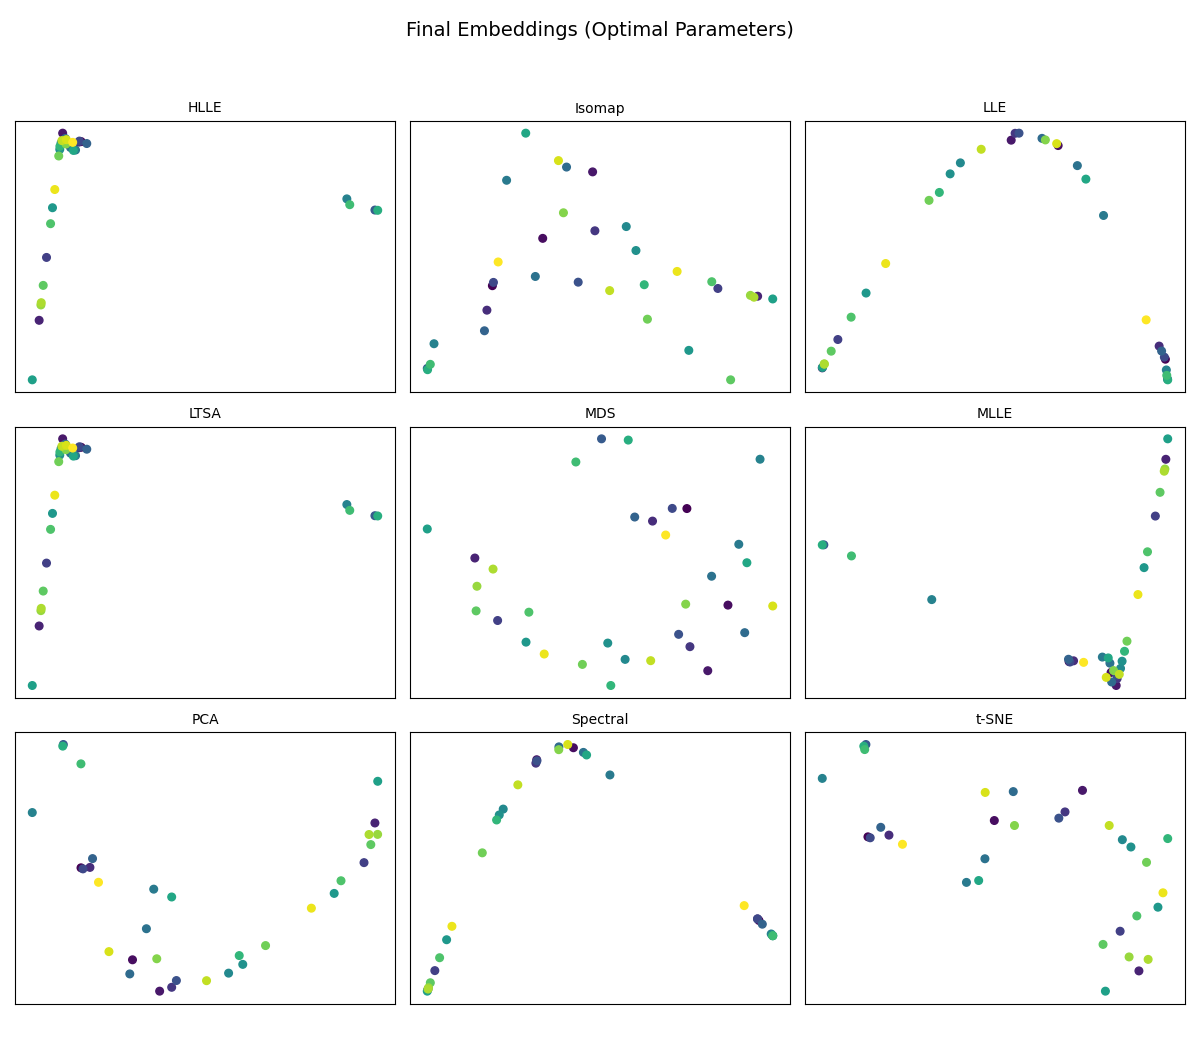
\includegraphics[width=0.8\linewidth]{../figs/final_scatter.png} % Using relative path
  \caption{Final 2D Embeddings (Scatter Plots) using optimal parameters.}
  \label{fig:final_scatter}
\end{figure}

% TODO: Insert Figure: Final Image Plot Grid (Cell 12 output)
\begin{figure}[htbp]
  \centering
  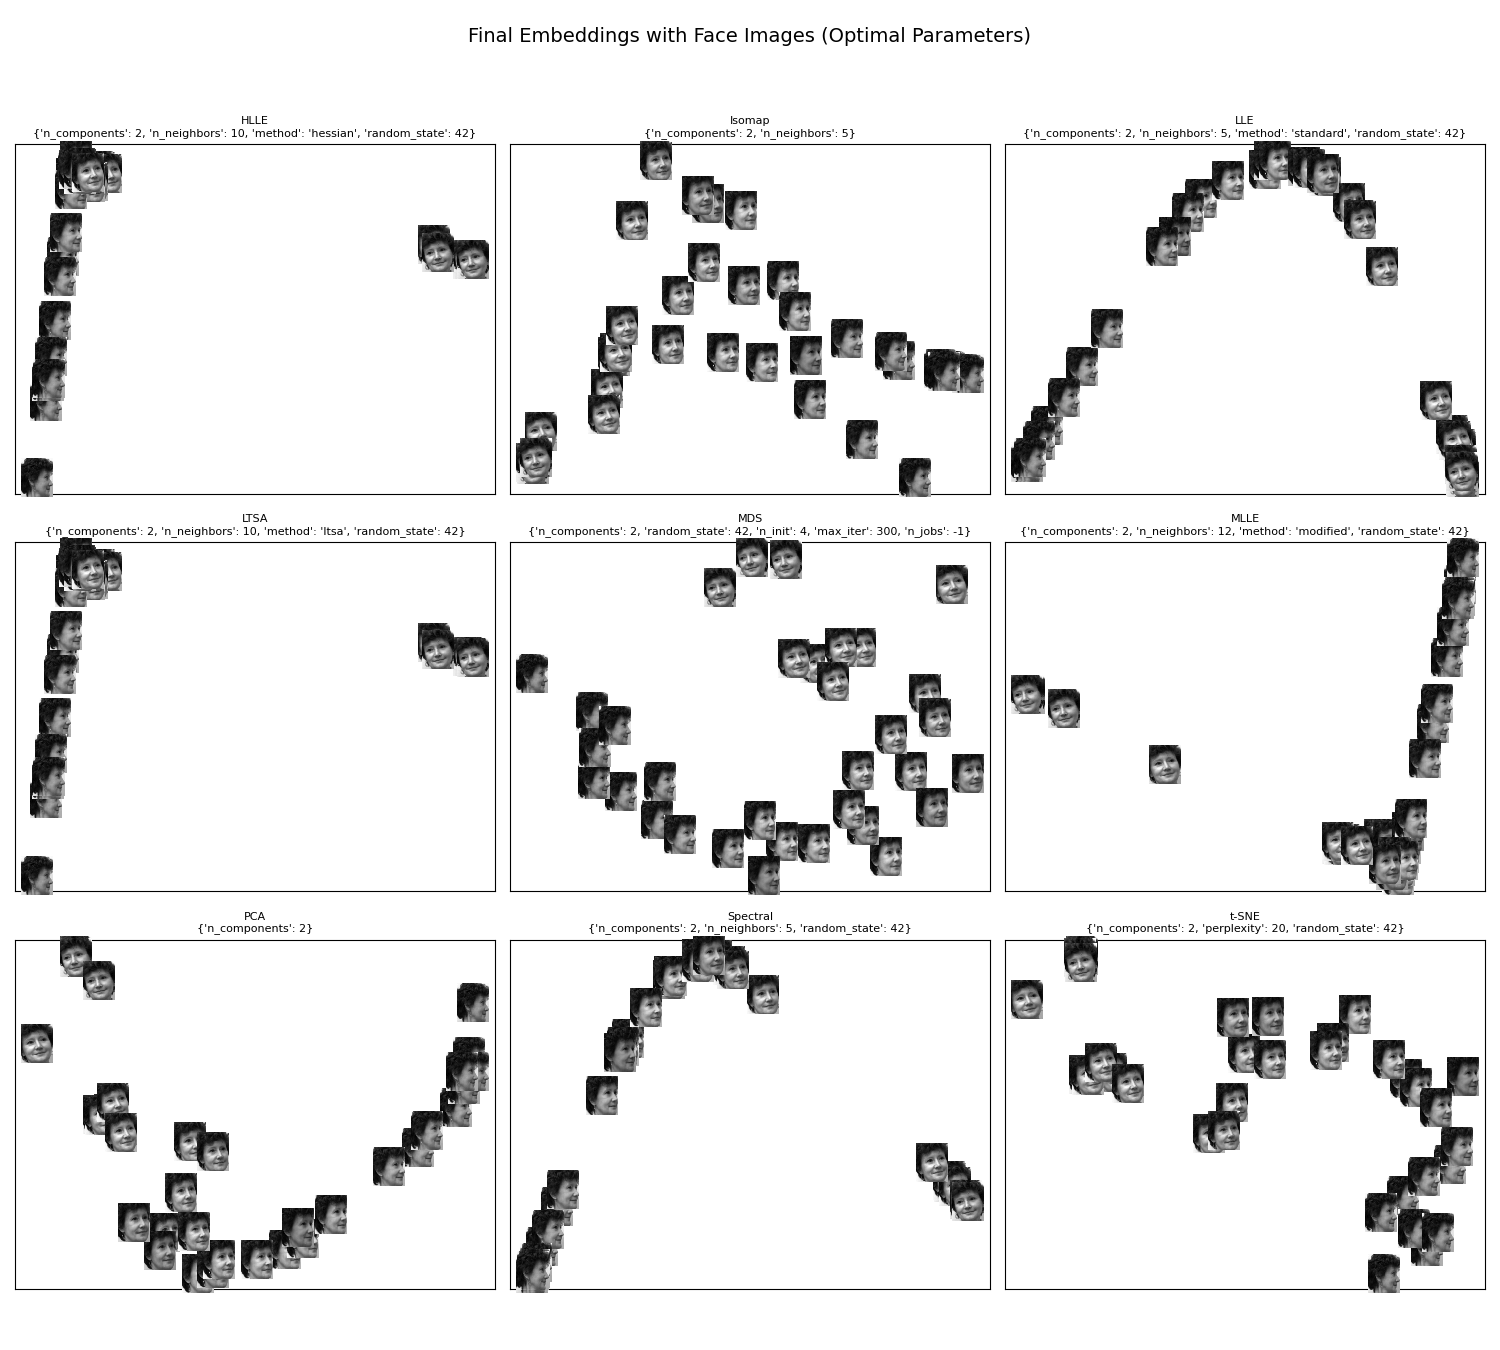
\includegraphics[width=0.8\linewidth]{../figs/final_images.png} % Using relative path
  \caption{Final 2D Embeddings with Face Images using optimal parameters.}
  \label{fig:final_images}
\end{figure}


\subsection{Parameter Tuning Analysis}
\label{sec:tuning}
% TODO: Discuss Figures 4 and 5 here.
The influence of the number of neighbors $k$ is shown in Figure \ref{fig:tuning_k}. Optimal TAE was mostly found for $k \in [5, 10]$. T\&C generally plateaued for $k \ge 5$.

% TODO: Insert Figure: Metrics vs k (Your refined k-tuning plot)
\begin{figure}[htbp]
  \centering
  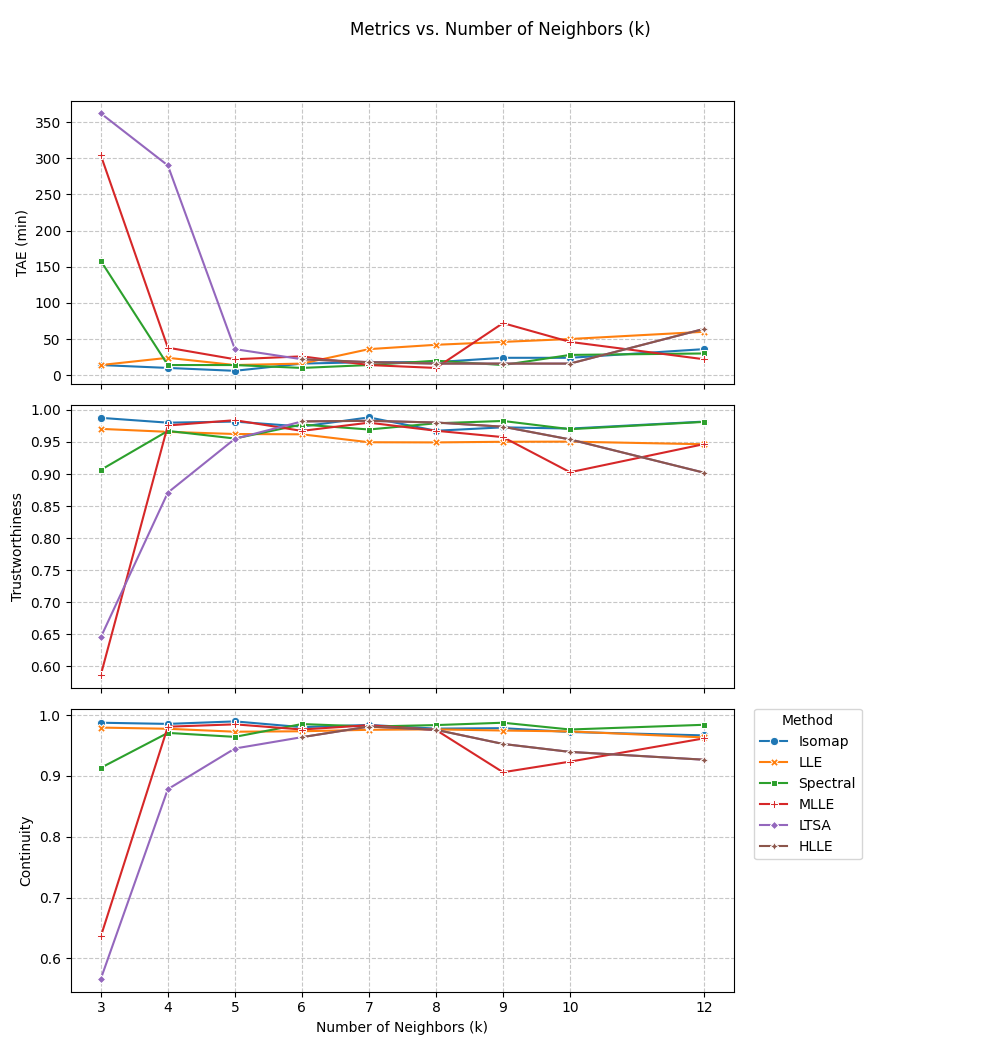
\includegraphics[width=0.75\linewidth]{../figs/tuning_k.png} % Using relative path
  \caption{Evaluation metrics versus number of neighbors (k).}
  \label{fig:tuning_k}
\end{figure}

The effect of perplexity $p$ on t-SNE (Figure \ref{fig:tuning_p}) showed optimal TAE at $p=20$, while T\&C were less sensitive.

% TODO: Insert Figure: Metrics vs Perplexity (Your perplexity tuning plot)
\begin{figure}[htbp]
  \centering
  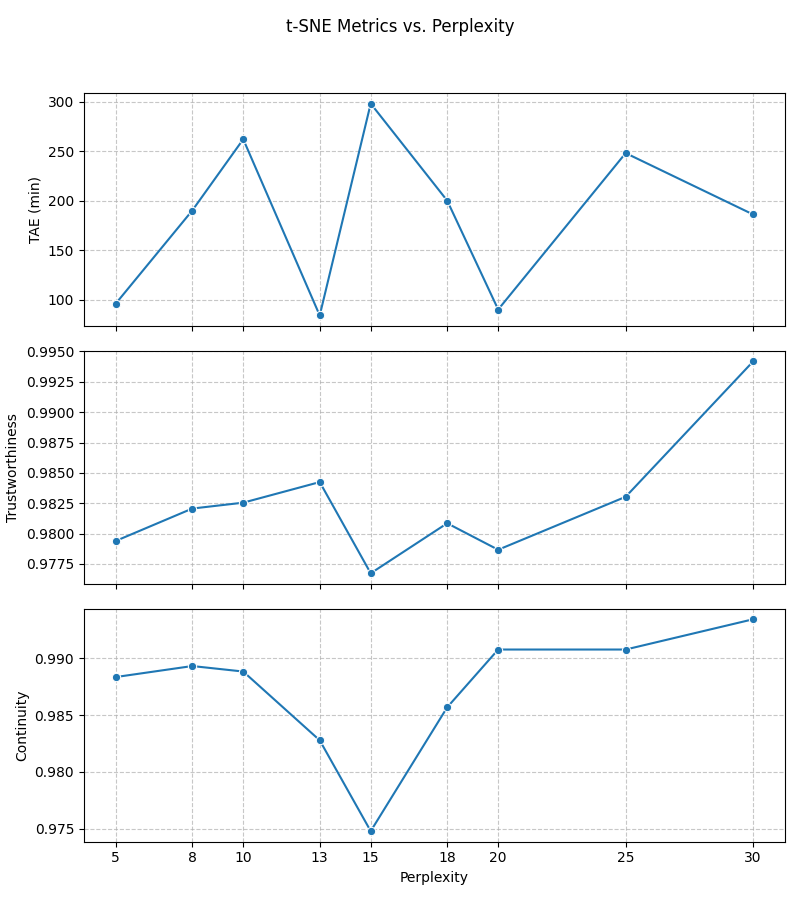
\includegraphics[width=0.7\linewidth]{../figs/tuning_p.png}
  \caption{t-SNE evaluation metrics versus perplexity (p).}
  \label{fig:tuning_p}
\end{figure}

\subsection{Discussion}
% TODO: Add your detailed discussion here.
% Compare methods, parameters, GT impact, comparison to senior report.
Our results demonstrate the effectiveness of several manifold learning algorithms, particularly Isomap, LLE, Spectral, HLLE, and LTSA, in recovering the 1D rotational manifold. The optimal parameters ($k \in [5, 10]$, $p=20$) were crucial for performance. The main discrepancy with the reference work \citep{CSIC5011_RefReport}, where LLE was solely optimal, likely stems from the differing ground truth sequences used, highlighting the sensitivity of TAE to this subjective choice. [Your further discussion points...]

% --- CONCLUSION ---
\section{Conclusion}
\label{sec:conclusion}
% TODO: Write your conclusion based on the discussion.
This project comparatively analyzed nine dimensionality reduction techniques for face pose ordering. Isomap (k=5) provided the best ordering accuracy based on our visually refined ground truth, closely followed by LLE (k=5), Spectral (k=5), HLLE (k=10), and LTSA (k=10). Parameter tuning confirmed optimal performance typically occurs for $k \in [5, 10]$. The study underscores the utility of manifold learning and the importance of parameter selection and ground truth definition.

% --- CONTRIBUTIONS Section ---
\section*{Contributions}

Ding Ding: Developed the core code structure for data processing, implementing the embedding algorithms, and defining evaluation metrics. Took the lead on drafting and composing the final report manuscript.

Zihao Zhang: Focused on refining the experimental setup, systematically tuning hyperparameters ($k$ and perplexity) for the manifold learning methods, and contributed to the generation of key visualizations for the report. Also assisted in initial data preprocessing steps.

Bingsong Gao: Contributed to the optimization of the codebase and performed validation of the evaluation metric implementations. Involved in the final refinement and proofreading of the report, and played a significant role in designing and preparing the presentation materials.

% --- REFERENCES ---
\FloatBarrier % Force all figures above this point to be placed before the bibliography
\nocite{*}
\bibliography{references} % Use this to generate bibliography from .bib file



\end{document}

